\documentclass[10pt]{article}
\usepackage[utf8]{inputenc}
\usepackage[usenames, dvipsnames]{xcolor}
\usepackage{tikz}
\usetikzlibrary{shapes}
\usepackage{amsmath}
\usepackage{amsthm}
\usepackage{amssymb}
\usepackage{graphicx}
\usepackage{tabto} 
\usepackage{inputenc}
\usepackage{fontenc}
\usepackage[french]{babel}
\usepackage{geometry}
\usepackage{fancyhdr}
\usepackage{hyperref}
\usepackage{tkz-tab}
\usetikzlibrary{calc,matrix}
\usepackage{enumerate}
\usepackage{manfnt}
\usepackage{nameref}
\usepackage{lastpage}
\usepackage{makeidx}
\usepackage{pgfplots}
\usepackage{listings}
\usepackage{tcolorbox}


\pagestyle{fancy}
\usepackage{lastpage}
\renewcommand{\headrulewidth}{1pt}
\fancyhead[L]{\rightmark}
\fancyhead[R]{}
\renewcommand\footrulewidth{1pt}
\fancyfoot[C]{Loris Parisot\\
	\textbf{Page \thepage/\pageref{LastPage}}}
\fancyfoot[R]{\today}
\fancyfoot[L]{Rapport de stage \\E.N.S Lyon \& U.C.B.L}
\setlength{\headheight}{2cm}
\lhead{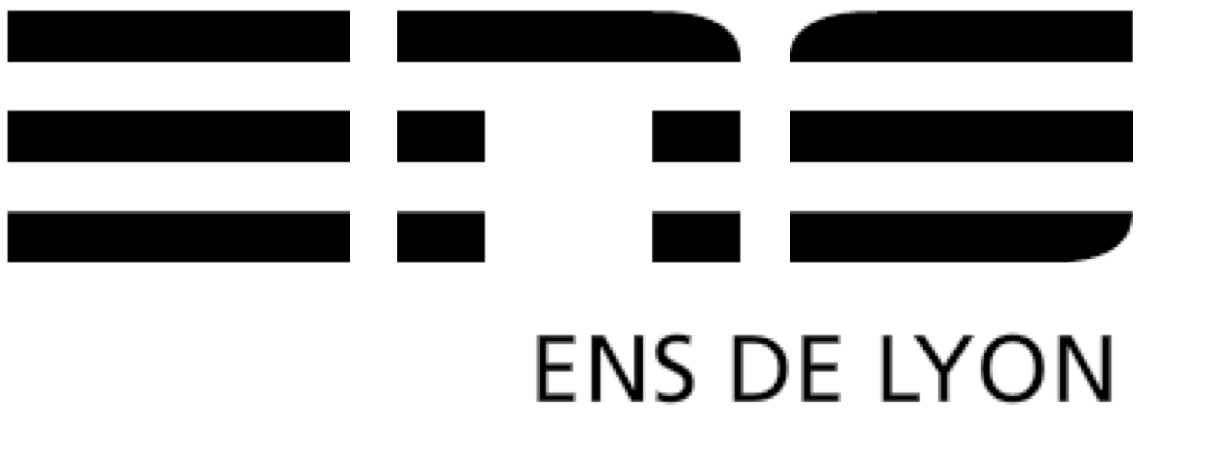
\includegraphics[scale=0.075]{figure/logo_ENS.jpg}}
\rhead{
\includegraphics[scale=0.075]{figure/logo_UCB.jpg}}

\newcommand{\fonction}[5]{\begin{array}{l|rcl}
		#1: & #2 & \longrightarrow & #3 \\
		& #4 & \longmapsto & #5 \end{array}}


\usepackage{color}
\definecolor{keywordcolor}{rgb}{0.7, 0.1, 0.1}   % red
\definecolor{tacticcolor}{rgb}{0.0, 0.1, 0.6}    % blue
\definecolor{commentcolor}{rgb}{0.4, 0.4, 0.4}   % grey
\definecolor{symbolcolor}{rgb}{0.0, 0.1, 0.6}    % blue
\definecolor{sortcolor}{rgb}{0.1, 0.5, 0.1}      % green
\definecolor{attributecolor}{rgb}{0.7, 0.1, 0.1} % red

\def\lstlanguagefiles{lstlean.tex}
% set default language
\lstset{language=lean}

\newtheorem{theoreme}{Théorème}
\theoremstyle{definition}
\newtheorem{lemme}[theoreme]{Lemme}
\newtheorem{definition}[theoreme]{Définition}
\newtheorem{corollaire}[theoreme]{Corollaire}
\newtheorem{proposition}[theoreme]{Proposition}
\newtheorem{propriete}[theoreme]{Propriété}
\newtheorem{application}[theoreme]{Application}
\newtheorem{exemple}[theoreme]{Exemple}
\newtheorem{remarque}[theoreme]{Remarque}


\newcommand{\revdots}{\reflectbox{$\ddots$}}
\DeclareMathOperator{\e}{e}
\DeclareMathOperator{\Dim}{dim}
\DeclareMathOperator{\Ker}{Ker}
\DeclareMathOperator{\rg}{rg}
\DeclareMathOperator{\spec}{Spec}



\newtcolorbox{mybox}[2][]{colback=red!5!white,
	colframe=red!75!black,fonttitle=\bfseries,
	colbacktitle=red!85!black,enhanced,
	attach boxed title to top center={yshift=-2mm},
	title={#2},#1}

\begin{document}
	\thispagestyle{empty} 
	
	
\includegraphics[width=0.27\textwidth]{figure/logo.png} 
	\hfill
	
\includegraphics[width=0.5\textwidth]{figure/logo_lyon11.png}\par\vspace{1cm}
	\begin{center}
	\Large \textbf{Master de Mathématiques Avancées}\normalsize \\
	\textsc{Parcours Higher Algebra and Formalization}\\ \vspace{8\baselineskip}
	\Huge \textbf{Rapport de stage} \normalsize \\ \vspace{0.9\baselineskip}
	\Large Loris PARISOT \normalsize\\ \vspace{2\baselineskip}
	\rule{0.95\textwidth}{2pt}\vspace{0.9\baselineskip}\\
	\LARGE \textbf{Formalisation de la représentation de Weil pour les groupes classiques sur corps finis en $\mathbf{L\exists\forall N}4$}\vspace{0.5\baselineskip}\normalsize\\
	\rule{0.95\textwidth}{2pt}\\
	\Large \textit{encadré par} Sophie MOREL
	\end{center}
	\vspace{10cm}
	\newpage
	\section*{Introduction}
	Ce stage de M2, réalisé à l'U.M.P.A et encadré par Sophie Morel, consistait en la formalisation des résultats issus de l'article \og Weil representations associated to finite fields \fg de Paul Gérardin. 
	\newline
	
	Au début du stage, certains prérequis à la formalisation de l'article n'existait pas dans mathlib. Il a donc fallu les implémenter avant de pouvoir travailler sur l'article, celui-ci devenant alors mineur par rapport aux prérequis à implémenter.
	\newline
	
	Voici un lien vers un site qui contient : le lien vers le git, le blueprint et le dependency graph.
	\url{https://lorisparisot.github.io/Weil_representations_associated_to_finite_fields/}
\newpage

\section{Formalisation informatique de preuve}

\subsection{L'assistant de preuve LEAN} 
La finalité de ce stage était la formalisation informatique de résultats (ainsi que de leurs preuves) de théorie des représentations. 
\newline

La formalisation informatique de preuves consiste grossièrement en traduire des énoncés mathématiques à ce qu'on appelle un \textit{assistant de preuve }dans un langage compréhensible par un ordinateur qui sera alors en mesure de dire si les énoncés ont un sens ou non et si leurs preuves sont exactes ou non. Il existe de nombreux assistants, les plus connus étant \textit{Rocq}, \textit{Isabelle} et \textit{LEAN} qui est celui qui a servi à ce projet.
\newline

Pour formaliser des résultats en \textit{LEAN}, il a été développé une bibliothèque, \textit{Mathlib}, regroupant tous les résultats déjà implémentés et pouvant être directement utilisés. Cette bibliothèque est collaborative : n'importe qui peut soumettre un résultat et sa preuve, qui fera alors l'objet (sur le même modèle que les publications classiques en mathématiques) d'une revue par les pairs qui déterminera si celui-ci est \og bien formalisée \fg : respect de la façon d'écrire, temps de compilation du code, est-il assez général,...
\textit{Mathlib} possède de plus une assez grande communauté dont les membres peuvent s'inscrire sur un forum en ligne pour discuter, demander de l'aide pour formaliser et prouver des résultats, etc.
\newline

L'interface du langage \textit{LEAN} sur le logiciel de codage \textit{VSCode} se présente en deux parties. Une première qui permet d'écrire du code, et une seconde permettant de voir les  objets mathématiques et les énoncés mis en jeu ainsi que le but de la preuve. \textit{LEAN} utilisant la correspondance de Curry-Howard, les propositions sont représentés par des types.

\subsection{Blueprint, une carte interactive pour formaliser}

\textit{Blueprint} est un outil développé spécialement pour les projets de formalisation en \textit{LEAN} par Patrick Massot. Il permet de déployer automatiquement une page web hébergée par Github sur laquelle on retrouve : 
\begin{itemize}
	\item [$\bullet$] Les fichiers associés au projet de formalisation
	\item[$\bullet$] Une documentation complète de \textit{Mathlib} avec les nouveaux résultats implémentés.
	\item [$\bullet$] Un fichier latex permettant d'écrire un article avec, pour chaque résultats, la possibilité d'ajouter un lien vers le résultat formalisé dans la documentation.
	\item[$\bullet$] Un graphe de dépendance des résultats implémentés, c'est-à-dire un graphe dont les sommets sont les noms des propositions et dont les arêtes indiquent les relations entre ces propositions. Le tout agrémenté d'un code couleur indiquant si le résultat est formalisé ou pas encore.
\end{itemize}

Cet outil a deux avantages majeurs. Le premier est qu'il permet de structurer le projet de formalisation et de s'organiser lors de travaux à plusieurs. Le second est qu'il a été pensé pour des mathématiciens souhaitant faire de la formalisation : il ne nécessite aucun pré requis informatique et se met en place assez facilement.


\section{Groupe d'Heisenberg}

\subsection{Convention}
L'article de P. Gérardin ne prend pas pour convention l'identification canonique de $V$ avec $V**$, mais la suivante : pour tout $(y,x)\in V^*\times (V^*)^* $, $\langle x, y\rangle = -\langle y,x\rangle = - y(x)$. 

Il suffit pour se faire de définir cette application linéaire dans \textit{LEAN}. Toute la machinerie sur le dual d'un espace vectoriel étant d'ors et déjà dans \textit{mathlib}, on peut s'en servir pour se faciliter une part de travail. Pour l'application réciproque, on utilise en particulier \lstinline|Module.evalEquiv k V| qui est la bijection canonique entre $V$ et $V^{**}$. Notre réciproque peut donc s'écrire \lstinline|fun x => - ((Module.evalEquiv k V).invFun (x))|, ce qui nous permet d'utiliser toute la machinerie derrière elle. L'application de $V$ dans $V^{**}$ est définie en utilisant la syntaxe \lstinline|- LinearMap.id.flip x|. 


\subsection{Groupe d'Heisenberg}

Considérons $\mathbb{K}$ un corps fini, $V$ un $\mathbb{K}-$espace vectoriel de dimension fini $n$ et $V^*$ son dual. On définit alors une structure de groupe sur les triplets $(z,x,y)\in\mathbb{K}\times V\times V^*$.

\definition{L'ensemble $H=\{(z,x,y)\in \mathbb{K}\times V\times V^*\}$ muni de $1:=(0,0,0)$ et de l'opération \\$\fonction{\star}{H\times H}{H}{((z_1,x_1,y_1),(z_2,x_2,y_2))}{(z_1+z_2+y_1(x_2), x_1+x_2,y_1+y_2)}$ forme un groupe appelé groupe d'Heisenberg associé à $V$ et noté $\mathcal{H}(V)$.}
 
\begin{center}
\begin{tcolorbox}[title = $L\exists\forall N$,width=12cm,text width=12cm,colback=lightgray!30,
	colframe=gray,sharp corners,
	rounded corners=uphill ]
	\begin{lstlisting}
		@[ext]
		structure Heisenberg (k V : Type*) [Field k] [Fintype k] [AddCommGroup V] [Module k V] where
		z : k
		x : V
		y : Module.Dual k V
		
		def Heisen_mul {k V : Type*} [Field k] [Fintype k] [AddCommGroup V] [Module k V]
		(H1 H2 : Heisenberg k V) : Heisenberg k V :=
		⟨H1.z + H2.z + (H1.y H2.x), H1.x + H2.x, H1.y + H2.y⟩
		
		def Heisen_mul_invdef {k V : Type*} [Field k] [Fintype k] [AddCommGroup V] [Module k V] (H : Heisenberg k V) : Heisenberg k V :=
		⟨ -H.z - (H.y (-H.x)), - H.x ,- H.y⟩
	\end{lstlisting}
\end{tcolorbox}
\end{center}

Notre article représente l'opération $\star$ par la multiplication matricielle sur des matrices $3\times3$, chose qui n'est pas possible en \textit{LEAN}, les matrices étant définies par 
\begin{center}
	\begin{tcolorbox}[title = $L\exists\forall N$,width=12cm,text width=12cm,colback=lightgray!30,
		colframe=gray,sharp corners,
		rounded corners=uphill ]
		\begin{lstlisting}
			def Matrix (m : Type u) (n : Type u') (α : Type v) : Type max u u' v :=
			m → n → α
		\end{lstlisting}
	\end{tcolorbox}
\end{center}
c'est-à-dire un tableau dont les lignes sont indexés par un type \lstinline|m|, des colonnes indexées par un type \lstinline|n| et dont les éléments sont tous de même type.
\newline

On montre alors aisément que  la formalisation proposée définie bien un groupe. L'ajout de \lstinline|[@ext]| permet d'obtenir automatiquement que si $H_1=H_2$, alors $x_1=x_2$, $y_1=y_2$ et $z_1=z_2$.
\newline

Une première déconvenue de cette façon de formaliser les choses est la non reconnaissance immédiate par $L\exists\forall N$ de la multiplication, de l'inverse et du $1$. Il est alors nécessaire d'appliquer à une hypothèse de la forme \lstinline|H1*H2=1| un \lstinline|change (Heinsen_mul H1 H2 = ⟨0, 0, 0⟩)| avant de pouvoir faire un \lstinline|rw| dessus, ce qui est loin d'être optimal.
\textit{Fixer le problème et mettre ça là}.
\newline

Deux théorèmes sur les groupes d'Heisenberg sont entre autres démontrés. Le premier stipule que $\mathcal{H}(V)$ est un groupe nilpotent d'ordre 2, c'est-à-dire $[\mathcal{H}(V),\mathcal{H}(V)]\ne\{1\}$ et $[\mathcal{H}(V),[\mathcal{H}(V),\mathcal{H}(V)]]=\{1\}$. 
\newline
Le second énonce que $\mathcal{H}(V)$ est anti-isomorphique à $\mathcal{H}(V^*)$.

\subsection{La tactique grind}

La formalisation des groupes d'Heisenberg a été l'occasion d'utiliser la tactique \lstinline|grind|. Le but de cette tactique est de clore automatiquement le goal, c'est-à-dire sans lui spécifier de quelle manière procéder. Elle utilise les même techniques que les solveurs SMT, \textit{Satisfiability Modulo Theories} qui sont des formules de premier ordre sans quantificateurs faisant intervenir des égalités. Le principe est le suivant : on construit la preuve en collectant toutes les données que l'on a faisant intervenir égalités, inégalités, booléens, puis dérive chacune de ces données (tout en gardant l'information principale), et ainsi de suite. On obtient alors une très grande quantité d'éléments, et but de la tactique est alors de clore le goal par contradiction.
\newline
Pour ce faire, \lstinline|grind| utilise les principes suivants :
\begin{itemize}
	\item [$\bullet$] \textit{Congruence closure} : on considère la cloture réflexive, transitive et symétrique de la relation \og est égal à\fg à laquelle on ajoute une égalité sur les fonctions \og si $a=b$ et $c=d$, alors $f\ a\ c= f\ b\ d$\fg. L'algorithme fusionne alors les classes d'équivalences jusqu'à arriver à un point fixe et essaye de trouver une contradiction. 
	\item [$\bullet$] \textit{Constraint propagation} : pour tout terme que \lstinline|grind| découvre via \textit{Congruence closure}, on lui applique des règles en plus : dérivation des booléens (par exemple si $A\wedge B$ vérifie \lstinline|True|, alors $A$ et $B$ sont également \lstinline|True|), projections (\lstinline|<x,y>=<a,b>| se dérive en \lstinline|x=a| et \lstinline|y=b|).
	\item[$\bullet$] \textit{Inductive Types} :  si dans les classes d'équivalences de \lstinline|grind| un même terme est formé par deux constructeurs différents d'un même type inductif, alors on obtient \lstinline|False| (par exemple $\forall$ et $\emptyset$). Si deux termes issus d'un même constructeur se retrouvent dans la même classe d'équivalence, alors on rend leurs arguments égaux.
	\item[$\bullet$] Des solveurs arithmétiques et sur des anneaux commutatifs.
\end{itemize}
Contrairement à la tactique \lstinline|aesop|, on ne peut voir ce que fait \lstinline|grind|. Ceci a un désavantage : la tactique n'est pas performante pour \og générer\fg une preuve mathématiques, dans le sens où elle ne permet pas à l'utilisateur d'avoir accès à la dite preuve.

\section{Représentation induite}

\subsection{Les représentations dans Mathlib}
Les représentations ont la particularité dans Mathlib de ne pas être implementées de manière uniforme. La librairie étant collaborative, les personnes y participant proposent des résultats en lien avec leurs domaines de prédilections, donnant lieu, dans le cas des représentations, à un certain hétéroclitisme.
\newline

La première façon de penser aux représentations est celle classiquement enseigné, à savoir un morphisme $\rho : G \rightarrow GL(V)$ où $V$ est un espace vectoriel sur un corps $k$. Toujours dans le soucis d'avoir une librairie la plus généraliste possible, on obtient dans Mathlib la définition suivante : \lstinline|Representation k G V = (G →* V →[k] V)| avec les instances \lstinline|[CommSemiring k] [Monoid G] [AddCommMonoid V] [Module k V]|.
\newline

Une autre façon de voir les représentations est d'utiliser un point de vue catégorique : en effet, on peut, étant donné un monoïde $G$ et un anneau $R$, introduire la catégorie des représentations $R-$linéaires de $G$ en prenant l'action de $G$ sur l'ensemble des modules finis sur $R$. On obtient la formalisation \lstinline|FDRep R G = Action (FGModuleCat R) G| où \lstinline|FGModuleCat R| désigne la catégorie des modules engendrés de manière finie.
\newline

Ces points de vue sont heureusement reliés entre eux via différents lemmes mais qui ont parfois tout de même des subtilités d'utilisation. Par exemple, le passage d'un élément de \lstinline|FDRep R G| à la définition via les morphismes se fait via \lstinline|FDRep.ρ| de manière immédiate en interprétant une représentation de $f$ de $G$ dans le $\mathbb{K}$-espace vectoriel $V$	comme un morphisme d'algèbres entre $\mathbb{K}[G]$ et les endomorphismes $\mathbb{K}-$linéaires de $G$ via $\fonction{\tilde{f}}{\mathbb{K}[G]}{\mathcal{L}_k(G)}{\sum\limits_{g\in G}a_gg}{\sum\limits_{g\in G}a_g f(g)}$. On définit alors la multiplication externe sur $V$ par $x\cdot v := (\tilde{f}(x))(v)$ pour tout $x\in \mathbb{K}[G]$ et tout $v\in V$.

\begin{center}
	\begin{tcolorbox}[title = $L\exists\forall N$,width=13cm,text width=13cm,colback=lightgray!30,
		colframe=gray,sharp corners,
		rounded corners=uphill ]
		\begin{lstlisting}
			/-- If `ρ : Representation k G V`, then `ρ.asModule` is a type synonym for `V`, which we equip with an instance `Module (MonoidAlgebra k G) ρ.asModule`.
			
			You should use `asModuleEquiv : ρ.asModule ≃+ V` to translate terms.
			-/
			
			@[nolint unusedArguments]
			def asModule (_ : Representation k G V) := V
			
			deriving AddCommMonoid, Module k
			
			/-- A `k`-linear representation of `G` on `V` can be thought of as a module over `MonoidAlgebra k G`.
			-/
			noncomputable instance : Module (MonoidAlgebra k G) ρ.asModule := Module.compHom V (asAlgebraHom ρ).toRingHom
		\end{lstlisting}
	\end{tcolorbox}
\end{center}

En revanche, si l'on veut passer du point de vue $\mathbb{K}[G]$ module au point de vue  morphisme, la situation est plus délicate. En effet, si $V$ est un $\mathbb{K}[G]$ module, il existe une multiplication externe $x\cdot v$ entre éléments de $\mathbb{K}[G]$ et de $V$ telle que $(xy)\cdot v=x\cdot(y\cdot v)$. On peut alors considérer l'action de $G$ sur $V$ définie par $\rho(g)(v)=g\cdot v$. L'application $g\mapsto \rho(g)(-)$ définie alors une représentation de $G$ dans $V$. C'est ce que fait \lstinline|Representation.ofModule'|. Le soucis de cette formalisation est qu'elle repose sur l'existence d'une instance \lstinline|Module k M| ainsi qu'une instance \lstinline|IsScalarTower k (MonoidAlgebra k G) M| (qui est une compatibilité des multiplications) qui est quelque chose d'immédiat mathématiquement mais pas en formalisation.
\newline

La manière choisie pour palier à ça est de définir une représentation non plus sur \lstinline|M|, mais sur \lstinline|RestricScalars k (MonoidAlgebra k G) M|. Si l'on souhaite mettre une structure de $R$ algèbre sur un anneau $S$, on a une équivalence de catégories entre la catégorie des $S-$modules et la catégorie des représentations de l'algèbre $S$ sur $R$ donnée par : à toute représentation $f$ de $S$ dans $\mathcal{L}_R(M)$, on associe le $S-$module $M$ avec l'action $s\cdot m := f(s)(m)$ et, réciproquement, à un $S-$module $M$ on définit une représentation $f(s)(m):=s\cdot m$. La formalisation de cette équivalence est \lstinline|RestricScalars R S M|. Ce dernier est équivalent à \lstinline|M|, mais se passe des instances précédemment requises. C'est donc celui-ci qui est généralement utilisé. Il est de plus l'inverse (au sens d'équivalence de catégories) de notre précédent \lstinline|Representation.asModule|.


\begin{center}
	\begin{tcolorbox}[title = $L\exists\forall N$,width=13cm,text width=13cm,colback=lightgray!30,
		colframe=gray,sharp corners,
		rounded corners=uphill ]
		\begin{lstlisting}
		/-- Build a `Representation k G M` from a `[Module (MonoidAlgebra k G) M]`.
		
		This version is not always what we want, as it relies on an existing `[Module k M]` instance, along with a `[IsScalarTower k (MonoidAlgebra k G) M]` instance.
		
		We remedy this below in `ofModule` (with the tradeoff that the representation is defined only on a type synonym of the original module.)
		-/
		noncomputable def ofModule' (M : Type*) [AddCommMonoid M] [Module k M]
		[Module (MonoidAlgebra k G) M] [IsScalarTower k (MonoidAlgebra k G) M] : Representation k G M :=
		(MonoidAlgebra.lift k G (M →ₗ[k] M)).symm (Algebra.lsmul k k M)
			
		/-- Build a `Representation` from a `[Module (MonoidAlgebra k G) M]`.
		
		Note that the representation is built on `restrictScalars k (MonoidAlgebra k G) M`,	rather than on `M` itself.
		-/
		noncomputable def ofModule : Representation k G (RestrictScalars k (MonoidAlgebra k G) M) :=
		(MonoidAlgebra.lift k G (RestrictScalars k (MonoidAlgebra k G) M →ₗ[k] RestrictScalars k (MonoidAlgebra k G) M)).symm	(RestrictScalars.lsmul k (MonoidAlgebra k G) M)
		\end{lstlisting}
	\end{tcolorbox}
\end{center}


On peut noter que ces points de vue différents peuvent mener à des utilisations \og non-optimales \fg. Par exemple, la notion de caractère d'une représentation est implémentée 


\subsection{Représentation induite}
L'article utilise la notion de représentation induite et celle de son caractères. Ces notions étaient étrangères à \textit{Mathlib} lorsque nos avons eu besoin de nous en servir, il a donc fallu les définir. Plusieurs options s'offrent alors à nous.
\newline

La première est de la définir ad hoc. Le problème de cette manière de procéder est qu'elle peut vite se révéler fastidieuse. Il est en effet bien plus aisé, lorsque l'on fait de la formalisation, de définir des objets puis de prouver des propriétés dessus plutôt que de les construire.
\newline

La deuxième option serait d'utiliser des notions de théorie des représentations déjà implémentés dans la librairie et plus particulièrement celle de coinduite. La coinduite est bla bla bla. Dans le cas des groupes finis, celle-ci est isomorphe à l'induite. Notre article ne traitant que de groupes finis, cela permettrait de s'économiser de la formalisation. En revanche, plus que de l'induite c'est de ses propriétés que nous avons besoin. Et la coinduite ne permet pas d'espérer formaliser facilement la réciprocité de Frobenius dont nous aurons besoin.
\newline

Vient ensuite la solution choisie, l'utilisation de l'algèbre de groupe : on se donne $G$ un groupe, $H$ un sous-groupe de $G$ et $\theta$ une représentation de $H$ dans un espace vectoriel $W$ sur un corps $\mathbb{K}$. Soit $W'$ le $\mathbb{K}[H]$ module associé à $\theta$. On construit $\rho$ la représentation de $G$ donnée par le $\mathbb{K}[G]$ module tensoriel $V:=\mathbb{K}[G]\otimes_{\mathbb{K}[H]}W$.
\newline 

Cette façon de traiter la représentation induite possède néanmoins un désavantage : elle utilise le produit tensoriel. En effet, $M\otimes N$ n'est défini que pour des modules $M$ et $N$ définis sur un même anneau commutatif. L'une des raisons de cette absence est la façon avec laquelle \textit{LEAN} fonctionne. 
\newline
Or, $\mathbb{K}[H]$ n'est a priori pas un anneau commutatif. En revanche, il est clair que si $H$ est un sous-groupe commutatif de $G$, alors $\mathbb{K}[H]$ est commutatif. Or, l'article de P. Gérardin se concentre sur des induites depuis le centre, donc depuis un sous-groupe commutatif. 
\newline

 Il s'agit ensuite de vérifier que cette représentation vérifie deux propriétés suivantes : 
 \begin{itemize}
 	\item [$\bullet$] $W\equiv\mathbb{K}[H]\otimes_{\mathbb{K}[H]}W$ est bien un sous $\mathbb{K}[H]$ module de $V$.
 	\item[$\bullet$] La réciprocité de Frobenius : si $E$ est un $\mathbb{K}[G]$ module, on a un isomorphisme entre $\text{Hom}_{\mathbb{K}[G]}(V,E)$ et $\text{Hom}_{\mathbb{K}[H]}(W,E)$.
 \end{itemize}

La preuve du premier point est une preuve calculatoire ne présentant pas spécialement de difficulté.
La preuve du second point utilise le lemme suivant : si $A$ est un un anneau commutatif, $B$ une $A-$algèbre, $M$ et $N$ deux $A-$modules, alors on a un isomorphisme $A-$linéaire $\text{Hom}_B(B\otimes_AM,N)\simeq \text{Hom}_A(M,N)$. Pour le montrer, on fourni une application $A-$linéaire et vérifie sa bijectivité, à savoir l'application $\fonction{\Psi}{\text{Hom}_B(B\otimes_AM)}{\text{Hom}_A(M,N)}{\varphi}{\fonction{\Psi_\varphi}{M}{N}{x}{\varphi(1\otimes_A x)}}$. Cette application est bien injective : si $\Psi_\varphi=\Psi_\phi$, alors pour tout $m\in M$, $\varphi(1\otimes_A m)=\phi(1\otimes_Am)$ et donc $\varphi=\phi$. Pour la surjectivité, on fabrique un antécédent explicite de l'application $B$ linéaire $\varphi:M\rightarrow N$ ainsi : on pose $\psi$ application $B$ linéaire de $B\otimes_A M$ dans $N$ définie par $\psi(b\otimes_Am)=b\varphi(m)$. Ainsi, on a bien $\Psi_\psi(x)=\psi(1\otimes_Ax)=\varphi(x)$ pour tout $x$ de $M$.
\newline

C'est ici que l'on voit tout l'intéret d'avoir choisi le point de vue de $\mathbb{K}[G]$ : la réciprocité de Frobenius devient une application de ce résultat deux fois : une première fois pour avoir l'isomorphisme $\text{Hom}_{\mathbb{K}[G]}(\mathbb{K}[G]\otimes_{\mathbb{K}[\mathcal{Z}_G]}W,E)\simeq\text{Hom}_{\mathbb{K}[\mathcal{Z}_G]}(W,E)$ et une seconde fois en prenant l'inverse de $\text{Hom}_{\mathbb{K}[\mathcal{Z}_G]}(\mathbb{K}[\mathcal{Z}_G]\otimes_{\mathbb{K}[\mathcal{Z}_G]} W)\simeq \text{Hom}_{\mathbb{K}[\mathcal{Z}_G]}(W,E)$
\newline

On obtient alors le résultat formalisé en seulement une ligne : 
\begin{center}
	\begin{tcolorbox}[title = $L\exists\forall N$,width=12cm,text width=12cm,colback=lightgray!30,
		colframe=gray,sharp corners,
		rounded corners=uphill ]
		\begin{lstlisting}
			noncomputable def iso_induced_as_tensor (E : Type*) [AddCommMonoid E] [Module (MonoidAlgebra k G) E] [Module (MonoidAlgebra k ↥(Subgroup.center G)) E] [inst6 : IsScalarTower (MonoidAlgebra k ↥(Subgroup.center G)) (MonoidAlgebra k G) E]:
			
			((tensor k G W θ) →ₗ[MonoidAlgebra k G] E) ≃ₗ[MonoidAlgebra k (Subgroup.center G)] ((module_sub_rep k G W θ) →ₗ[MonoidAlgebra k (Subgroup.center G)] E) := by
			
			exact ((iso_hom_tens (MonoidAlgebra k ↥(Subgroup.center G)) (θ.asModule) E (MonoidAlgebra k G)).trans (iso_hom_tens (MonoidAlgebra k ↥(Subgroup.center G)) θ.asModule E
			(MonoidAlgebra k ↥(Subgroup.center G))).symm)
			
		\end{lstlisting}
	\end{tcolorbox}
\end{center}


 
 
\subsection{Caractère de l'induite}
Le but de cette section est de formaliser le fait que \og le caractère de l'induit est l'induit du caractère\fg.
\newline

Etant donnée $f$ une fonction centrale sur un sous-groupe $H$ d'un groupe $G$, on définit l'induit de $f$ par la fonction $F_f$ définie par $F_f(s)=\frac{1}{Card(H)}\sum\limits_{t\in G \ \wedge \ t^{-1}st\in H}f(t^{-1}st)$ pour tout $s$ dans $G$. La fonction $F_f$ est alors une fonction centrale sur $G$.
\newline

La notion de fonction centrale étant absente de Mathlib, on la formalise ainsi : 

\begin{center}
	\begin{tcolorbox}[title = $L\exists\forall N$,width=12cm,text width=12cm,colback=lightgray!30,
		colframe=gray,sharp corners,
		rounded corners=uphill ]
		\begin{lstlisting}
			class conj_class_fun where
			Fun :  G → W
			conj_property : ∀ (x : G), ∀ (g : G), Fun (g⁻¹ * x * g) = Fun x
			
		\end{lstlisting}
	\end{tcolorbox}
\end{center}
Dans le but de formaliser le résultat escompté, il faut introduire la décomposition $\mathbb{K}[G]\equiv \bigoplus\limits_{i=1}^rg_i\cdot\mathbb{K}[\mathcal{Z}_G]$ où $(g_i)_{i\in[\!|1,r|\!]}$ désigne un système de représentant de $G/\mathcal{Z}_G$.
\newline
L'algèbre d'un groupe fini est la donnée de trois éléments : un groupe fini d'ordre $n$, un espace vectoriel $V$ de dimension $n$ et d'une base $(\e_g)_{g\in G}$ de $V$ indexée par $G$. Dans \textit{Mathlib}, on définit cet objet via \lstinline|MonoidAlgebra k G := G →₀ k|, c'est-à-dire par les applications à support fini de $G$ dans $k$.
\newline
Pour montrer cette décomposition, on introduit certains résultats sur les groupes et leur quotient par leur centre. On définit un système de représentant de $G$ par l'image de l'application $g\mapsto \bar{g}$ et on lui associe deux autres application : une qui envoie un élément sur son représentant, et une autre $g\mapsto h$ où $g=\bar{g}h$. :

\begin{center}
	\begin{tcolorbox}[title = $L\exists\forall N$,width=12cm,text width=12cm,colback=lightgray!30,
		colframe=gray,sharp corners,
		rounded corners=uphill ]
		\begin{lstlisting}
			abbrev set: Set G := by
			exact Set.range (@Quotient.out G (QuotientGroup.con (Subgroup.center G)).toSetoid )
			
			noncomputable def G_to_syst: G → ↑(system_of_repr_center.set G) := by
			intro g
			unfold system_of_repr_center.set
			refine ⟨ Quotient.out (Quotient.mk ((QuotientGroup.con (Subgroup.center G)).toSetoid) g), by simp⟩
			
			noncomputable def G_to_center : G → Subgroup.center G := by
			intro u
			exact ((QuotientGroup.mk_out_eq_mul (Subgroup.center G) u).choose)⁻¹
		\end{lstlisting}
	\end{tcolorbox}
\end{center}
Le principal avantage de mettre en place cette machinerie est de pouvoir implémenter différents lemmes \lstinline|simp| reliant ces applications et s'en servir pour simplifier des expressions. Cela permet également d'avoir des notations plus compactes et lisibles.
\newline

La preuve de la décomposition s'effectue en deux temps. On montre d'abord qu'on a un isomorphisme entre $\mathbb{K}[\mathcal{Z}_G]$ et $g\cdot \mathbb{K}[\mathcal{Z}_G]$ avec $g$ un élément du système de représentant de $G/\mathcal{Z}_G$, ce qui est obtenu via l'application $x\mapsto gx$. 
\newline
On montre ensuite que les éléments du système de représentants vus comme élément de $\mathbb{K}[G]$ forment une base de $\mathbb{K}[G]$ en tant que $\mathbb{K}[\mathcal{Z}_G]$ algèbre. La preuve n'a rien de bien compliqué sur le papier : une interversion de somme finie. Cependant, l'implémentation en \textit{LEAN} est un peu plus fastidieuse à cause de la gymnastique entre éléments de $\mathbb{K}[\mathcal{Z}_G]$, $\mathbb{K}[G]$ et $G$. 
On donne ensuite explicitement les applications liant $\mathbb{K}[G]$ et $\bigoplus\limits_{i=1}^rg_i\cdot\mathbb{K}[G]$, à savoir ...
 Pour implémenter la première, on utilise  un lemme sur les sommes directes : 
\begin{center}
	\begin{tcolorbox}[title = $L\exists\forall N$,width=12cm,text width=14cm,colback=lightgray!30,
		colframe=gray,sharp corners,
		rounded corners=uphill ]
		\begin{lstlisting}
			theorem DirectSum_eq_sum_direct (ι : Type*) [hi : Fintype ι] (β : ι → Type w)	[(i : ι) → AddCommMonoid (β i)] [DecidableEq ι] (x : (i : ι) → β i) 
			(j : ι) : (∑ (i : ι), (DirectSum.of β i) (x i)) j = x j  := by
			have := Finset.sum_apply (a := j) (g := fun i ↦ (DirectSum.of β i) (x i)) (s := Finset.univ)
			rw [DFinsupp.finset_sum_apply, Finset.sum_eq_single j]
			· simp only [DirectSum.of_eq_same]
			· intro a _ ha
			exact DirectSum.of_eq_of_ne _ _ _ ha
			· simp only [Finset.mem_univ, not_true_eq_false, DirectSum.of_eq_same, IsEmpty.forall_iff]
		\end{lstlisting}
	\end{tcolorbox}
\end{center}
Ce lemme est intéressant, dans le sens où sa preuve ne se comporte pas comme l'on aimerait qu'elle se comporte. L'énoncé est assez simple, la preuve est assez longue. Mais si l'on rajoute un \lstinline|simp[DirectSum]|, alors on peut clore le but directement via \lstinline|exact Fintype.sum_dite_eq j fun j_1 h ↦ Eq.symm h ▸ x j_1|. 
\begin{center}
	\begin{tcolorbox}[title = $L\exists\forall N$,width=12cm,text width=14cm,colback=lightgray!30,
		colframe=gray,sharp corners,
		rounded corners=uphill ]
		\begin{lstlisting}
		theorem DirectSum_eq_sum_direct (ι : Type*) [hi : Fintype ι] (β : ι → Type w)
		[(i : ι) → AddCommMonoid (β i)] [DecidableEq ι] (x : (i : ι) → β i) (j : ι) :
		(∑ (i : ι), (DirectSum.of β i) (x i)) j = x j  := by
		simp[DirectSum]
		exact Fintype.sum_dite_eq j fun j_1 h ↦ Eq.symm h ▸ x j_1
		\end{lstlisting}
	\end{tcolorbox}
\end{center}
Or, \lstinline|DirectSum| est implémenté dans \textit{Lean} comme étant \lstinline|Π₀ i, β i|, c'est-à-dire une fonction dépendante à support fini. Il n'y a donc a priori aucune raison que \lstinline|simp| n'arrive pas à ouvrir la définition. La raison de ce blocage est le manque de lemme à propos des sommes directes.

On arrive finalement au lemme suivant : 
\begin{center}
	\begin{tcolorbox}[title = $L\exists\forall N$,width=12cm,text width=14cm,colback=lightgray!30,
		colframe=gray,sharp corners,
		rounded corners=uphill ]
		\begin{lstlisting}
		/--Given a representative system `system_of_repr_center.set G` of `G⧸ (Subgroup.center G)`,
		we have a `MonoidAlgebra k (Subgroup.center G)` linear bijection between
		`MonoidAlgebra k G` and the direct sum of `g • (MonoidAlgebra k (Subgroup.center G))` for `g : system_of_repr_center.set G`.-/
		
		noncomputable def MonoidAlgebra_direct_sum_system_of_repr_center_set : MonoidAlgebra k G ≃ₗ[MonoidAlgebra k (Subgroup.center G)] DirectSum (system_of_repr_center.set G) (fun g => gkH_set k G g) := by
		
		have := DirectSum_equiv_linearmap (MonoidAlgebra k (Subgroup.center G)) (system_of_repr_center.set G) (fun g => gkH_set k G g) (fun g => MonoidAlgebra k (Subgroup.center G)) 	(fun g => (gkH_set_iso_kH_module k G g))
		exact LinearEquiv.trans (MonoidAlgebra_direct_sum_1 k G) this.symm
		\end{lstlisting}
	\end{tcolorbox}
\end{center}



\end{document}